\chapter{Literature}
\label{ch:background}

This chapter introduces technical concepts and background used in the conceptualized solution of the thesis.

\subsection{Sound Propagation}

Sound propagation is the physical process by which sound waves propagate in a given environment. The strength of the sound wave is dependent on a variety of factors, including the frequency, environment, and distance from the sound source. This makes it difficult to accurately identify and localize a sound source, and thus a more accurate and robust sound source localization system is needed.

\subsection{Realistic sound propagation in simulations}

\subsubsection{Microsoft Project Acoustics}

Microsoft Project Acoustics is a sound propagation engine that simulates the propagation of sound waves in a given environment. It is used in a variety of applications, including video games, virtual reality, and augmented reality. It simulates wave effects like obstruction, reverberation and occlusion in complex 3D scenes without requiring zone markup or raytracing. It works similarly to a raytracing engine, but it is precomputed and optimized for real-time performance. 



\subsection{Sound Propagation in game-engine}

\section{Sound Source Localization}

Sound Source Localization (SSL) is the process of determining the position of a sound source. This is usually done using a microphone array that captures the sound signals from multiple directions. SSL is used in a variety of applications, such as speech recognition, robot navigation, surveillance, and security. In this thesis, SSL is used to estimate the distance and direction of a sound source to detect excessively noisy vehicles.

\subsection{Spectrograms for sound source localization}

Spectrograms are a visual representation of the frequency content of a sound signal. They are often used in sound source localization to identify the direction of a sound source. The spectrogram is a two-dimensional representation of the frequency content of a sound signal. 

\begin{figure}[h]
    \centering
    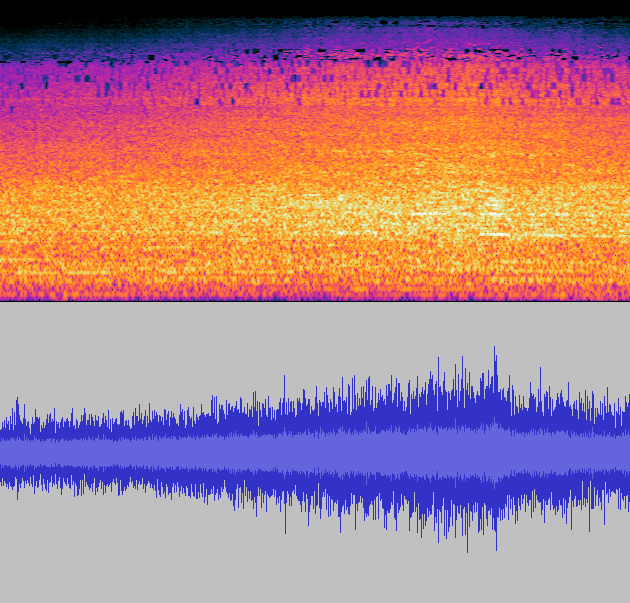
\includegraphics[width=0.5\textwidth]{../images/spectrogram.png}
    \caption{Spectrogram of a sound signal}
    \label{fig:spectrogram}
\end{figure}

The x-axis represents time and the y-axis represents frequency. The intensity of the color at each point in the spectrogram represents the amplitude of the frequency component then. The spectrogram can be used to identify the direction of a sound source by looking at the frequency content of the sound signal. The frequency content of a sound signal is dependent on the direction of the sound source, so the spectrogram can be used to identify the direction of a sound source.

\subsection{Convolutional Neural Networks}

\subsection{Convolutional Neural Networks for source localization}

\begin{figure}[h]
    \centering
    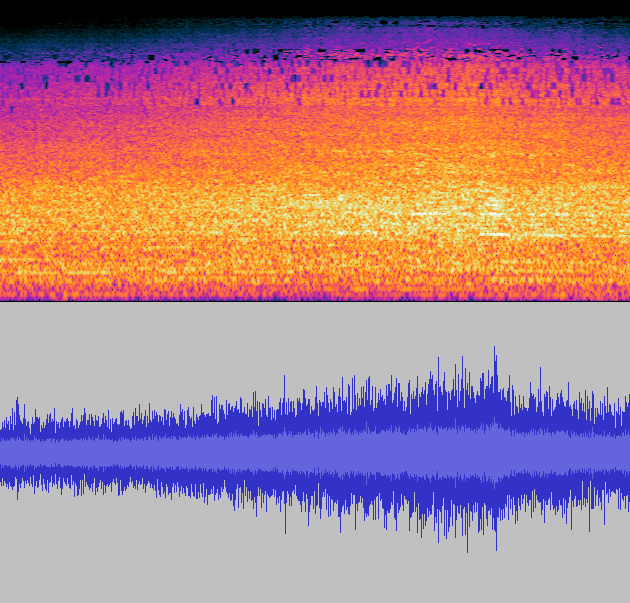
\includegraphics[width=0.5\textwidth]{../images/spectrogram.png}
    \caption{CNN sound classification diagram}
    \label{fig:cnn_sound_classification}
\end{figure}

\section{Related Work}

\subsection{}

